El modelo ARIMA o modelo autorregresivo de media móvil integrado, por sobre otros modelos de series temporales, se centra en describir las autocorrelaciones que existen entre los datos \cite{forecast-time-series-arima}.

\begin{itemize}
    \item \textbf{Estacionariedad:} Una serie de tiempo estacionaria, se presenta cuando sus propiedades no dependen del momento en el que fue registrada la observación. Por lo que, las series de tiempo que presentan tendencias o patrones estacionales son series de tiempo no estacionarias, ya que las tendencias y las distintas estaciones de tiempo pueden afectar la serie de tiempo en varias ocasiones \cite{forecast-time-series-arima}. 
    
    Las series de tiempo estacionarias por lo general son series de ruido blanco, ya que no muestran autocorrelación entre los datos y tampoco presentan patrones predecibles a lo largo del tiempo. 

    \item \textbf{Diferenciación:} Una manera de poder cambiar una seria de tiempo no estacionaria en una estacionaria, es aplicar la diferenciación, esto se refiera a calcular la diferencia entre observaciones consecutivas \cite{forecast-time-series-arima}.
    
    Una de las transformaciones más ocupada para estabilizar la varianza de los datos son los logaritmos. Por otro lado, la diferenciación estabiliza el promedio de la seria de tiempo debido a que es capaz de reducir o remover los distintos cambios que se puedan presentar en la serie de tiempo, tales como las tendencias y patrones estacionales.
    
    \item \textbf{Modelo Random walk:} La serie diferenciada es el cambio que se presenta entre las observaciones consecutivas de la serie original, esta se denota por:
    \begin{equation*}
        y'_t = y_t - y_t-1
    \end{equation*}

    Ya que es imposible conseguir la diferenciada de la primera observación $y'_1$, la serie diferenciada solo tendrá valores T-1. Si la serie diferenciada es un ruido blanco, la fórmula se puede escribir de la siguiente manera, donde $\varepsilon_t$ representa el ruido blanco \cite{forecast-time-series-arima}:
    \begin{equation*}
        y_t-y_t-1= \varepsilon_t
    \end{equation*}

    El \textbf{Modelo Random walk} se obtiene luego de despejar $y_t$:
    \begin{equation*}
        y_t=y_t-1+\varepsilon_t
    \end{equation*}

    Debido a que los movimientos futuros en los datos son impredecibles, las predicciones del modelo son iguales a la ultima observación, por lo que este tipo de modelos es ampliamente ocupado por datos no estacionarios. Pudiendo concluir que el modelo random walk sustenta los pronósticos naïve \cite{forecast-time-series-arima}.

    \begin{equation*} y_t-y_t-1 = C+\varepsilon_t \leftrightarrow y_t=C+y_t-1+\varepsilon_t \end{equation*}

    El valor de C representa el promedio de los cambios entre observaciones consecutivas \cite{forecast-time-series-arima}, dependiendo del signo de C la seria se verá derivada positivamente si es positivo o negativamente en el caso contrario.

    \item \textbf{Diferenciación estacional:} Esta diferenciación se realiza para calcuar el cambio entre una observación y la observación previa de la misma estación de tiempo \cite{forecast-time-series-arima}, obteniendo la siguiente fórmula:
    \begin{equation*}
        y'=y_t-y_t-m
    \end{equation*}

    Donde $m= \text{cantidad de estaciones}$, tambien son llamadas "diferencias $m$-desfazadas", ya que realizamos la resta con una observación luego de $m$ periodos \cite{forecast-time-series-arima}.

    Si luego de realizar una diferenciación estacional a una serie de tiempo, esta parece haberse transformado a ruido blanco, se modelaran los datos originales de la siguiente manera:
    \begin{equation*}
        y_t=y_t-m+\varepsilon_t
    \end{equation*}

    Como este tipo de modelo entrega predicciones iguales a la ultima observación de la estacion seleccionada, en otras palabras, este modelo entrega pronósticos naïve \cite{forecast-time-series-arima}.

    En la siguiente figura se muestra como las diferenciaciones estacionales y la aplicacion de logaritmos a una serie de tiempo, en este caso la venta de medicamentos antidiabéticos, lograr cambiar la forma de la serie a una de ruido \cite{forecast-time-series-arima}:

    \begin{figure}[H]
        \begin{minipage}[t]{0.9\textwidth}
            \caption{Aplicación de logartimos y diferenciación estacional a ventas de medicamentos antidiabéticos}
            \label{seasonaldiff}        
        \end{minipage}
    
        \vspace{10pt}
    
        \begin{minipage}[b]{1.1\textwidth}
            \centering
            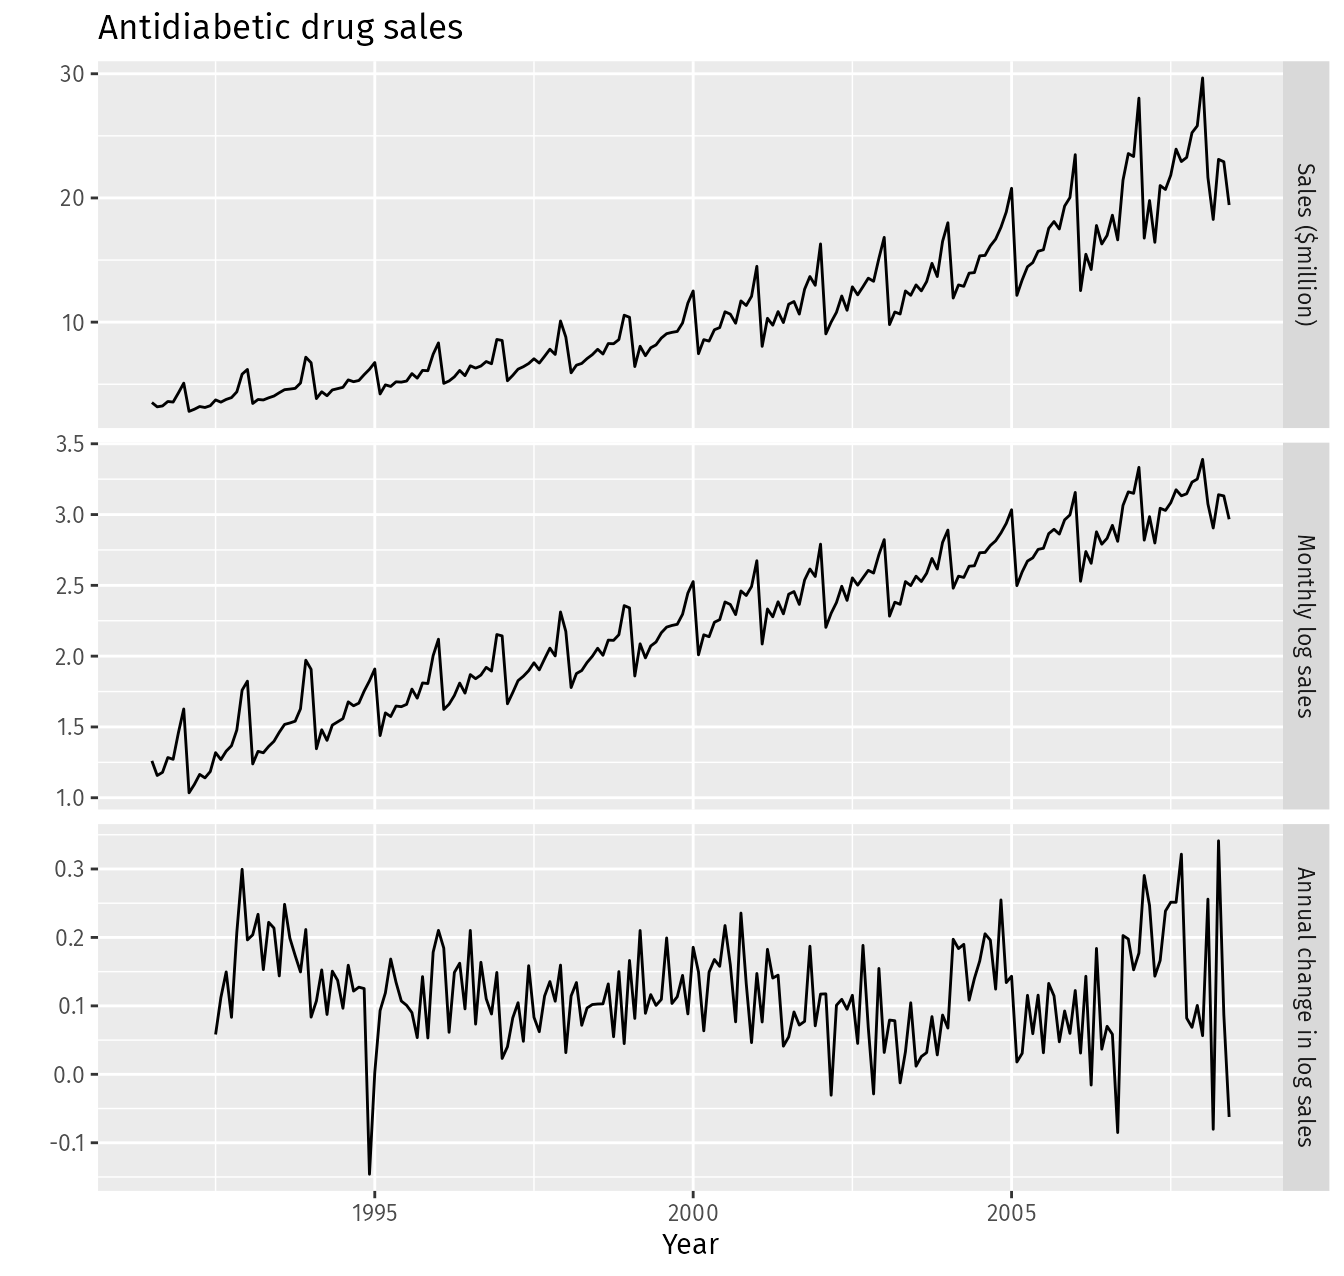
\includegraphics[width=\textwidth]{img/a10diff-1-seasonaldiff-example.png}        
        \end{minipage}
    
        \begin{minipage}[t]{0.9\textwidth}
            Fuente: Forecasting: Principles and Practice (Hyndman y Athanasopoulos, 2023). Recuperado de \url{https://otexts.com/fpp2/time-plots.html}
        \end{minipage}
    \end{figure}

    Por lo general, a la diferenciación ordinaria se le llama "primera diferenciación", refiriendose a las diferenciación en el desfase 1. 
    
    Para poder obtener una serie de tiempo que parezca ruido blanco, muchas veces se tendra que aplicar ambas diferenciaciones, la primera diferenciación y diferenciación estacional, el orden de aplicación no afecta el resultado \cite{forecast-time-series-arima}.
    
    Tambien existe la segunda diferenciada estacional, por lo que el modelo de la serie doblemente diferenciado se escribe de la siguiente manera:
    \begin{equation*}
        y''_t=y'_t-y'_t-1 \leftrightarrow (y_t-y_t-m)-(y_t-1-y_t-m-1) \leftrightarrow y_t-y_t-1-y_t-m+y_t-m-1
    \end{equation*}

    Si la serie de tiempo, presenta un patrón estacional, es recomendable realizar la diferenciación estacional como primer paso para obtener una serie de tiempo estacionaria, pero si se ocupa la primera diferenciación puede que todavia hayan patrones estacionales en la serie de tiempo, teniendo que aplicar más diferenciaciones para obtener la estacionariedad \cite{forecast-time-series-arima}.

    \item \textbf{Modelo de autorregresión:} Como se menciono anteriormente, los modelos autorregresivos predicen la variable de interes utilizando una combinación lineal de valores pasados de la variable. El término autorregresión indica que se trata de una regresión de la variable contra sí misma.
    
    Por lo que un modelo autorregresivo de orden $p$, donde $\varepsilon_t$ corresponde a ruido blanco, se escribe de la siguiente manera:
    \begin{equation*}
        y_t=c+\phi_1y_t-1+\phi_2y_t-2+...+\phi_py_t-p+\varepsilon_t
    \end{equation*}

    Este tipo de modelo es llamado \textbf{AR($p$)}, gracias a la flexibilidad de los modelos autorregresivos, estos pueden ser aplicados en series de tiempo que presenten distintos patrones \cite{forecast-time-series-arima}. A continuación, se presenta una figura que muestran dos modelos AR, AR(1) y AR(2).

    \begin{figure}[H]
        \begin{minipage}[t]{0.9\textwidth}
            \caption{Modelos autorregresivos con diferentes parámetros}
            \label{ARmodel}        
        \end{minipage}
    
        \vspace{10pt}
    
        \begin{minipage}[b]{1.1\textwidth}
            \centering
            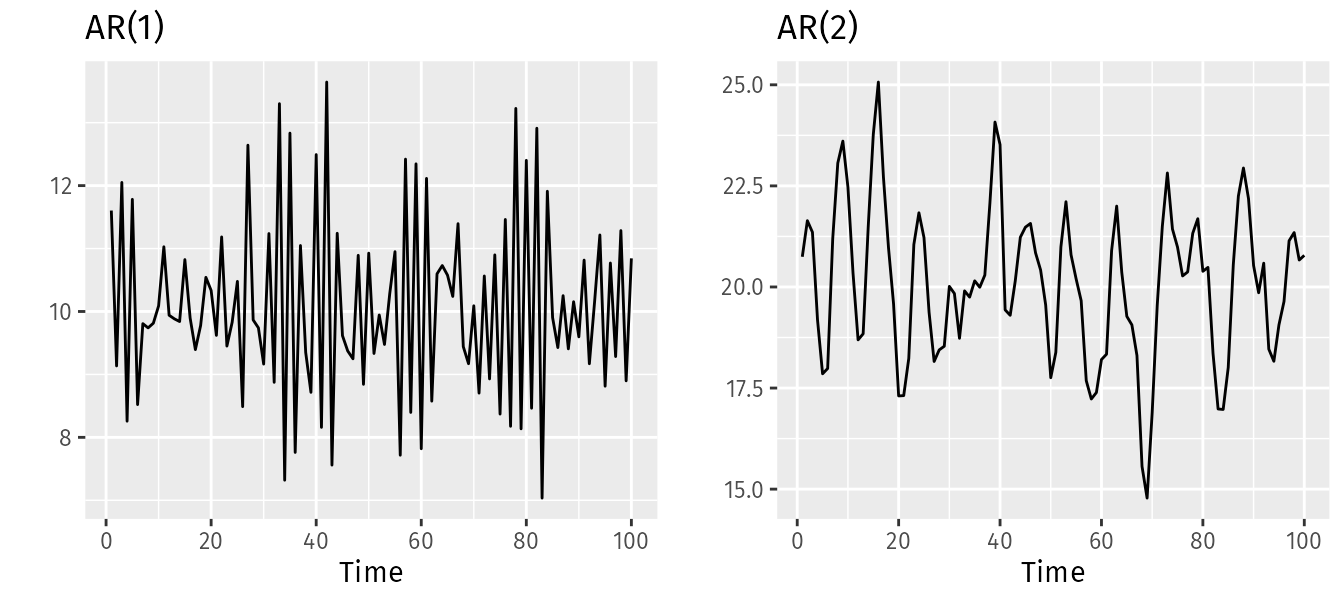
\includegraphics[width=\textwidth]{img/arp-1-example.png}        
        \end{minipage}
    
        \begin{minipage}[t]{0.9\textwidth}
            Fuente: Forecasting: Principles and Practice (Hyndman y Athanasopoulos, 2023). Recuperado de \url{https://otexts.com/fpp2/time-plots.html}
        \end{minipage}
    \end{figure}

    El modelo AR(1) tiene como fórmula: $y_t=18-0.8y_t-1+\varepsilon_t$ y el modelo AR(2) tiene como fórmula: $y_t=8+1.3y_t-1 - 0.7y_t-2+\varepsilon_t$, en ambos casos $\varepsilon_t$ (ruido blanco) tiene una distribución normal, con promedio igual a 0 y varianza igual a 1 \cite{forecast-time-series-arima}.

    \item \textbf{Modelo de media móvil:} Este tipo de modelo ocupa el error de los pronósticos como si fuera un modelo de regresión, con la diferencia en una regresión se ocupan los valores pasados. 

    Teniendo $\varepsilon_t$ como ruido blanco, el modelo de media móvil de orden $q$ o \textbf{MA($q$)} se escribe de la siguiente manera \cite{forecast-time-series-arima}:
    \begin{equation*}
        y_t=c+\varepsilon_t+\theta_1\varepsilon_t-1+\theta_2\varepsilon_t-2+...+\theta_q\varepsilon_t-q+\varepsilon_t
    \end{equation*}

    A continuación, se presenta una figura que muestran dos modelos MA, MA(1) y MA(2).

    \begin{figure}[H]
        \begin{minipage}[t]{0.9\textwidth}
            \caption{Modelos de media móvil con diferentes parámetros}
            \label{MAmodel}        
        \end{minipage}
    
        \vspace{10pt}
    
        \begin{minipage}[b]{1.1\textwidth}
            \centering
            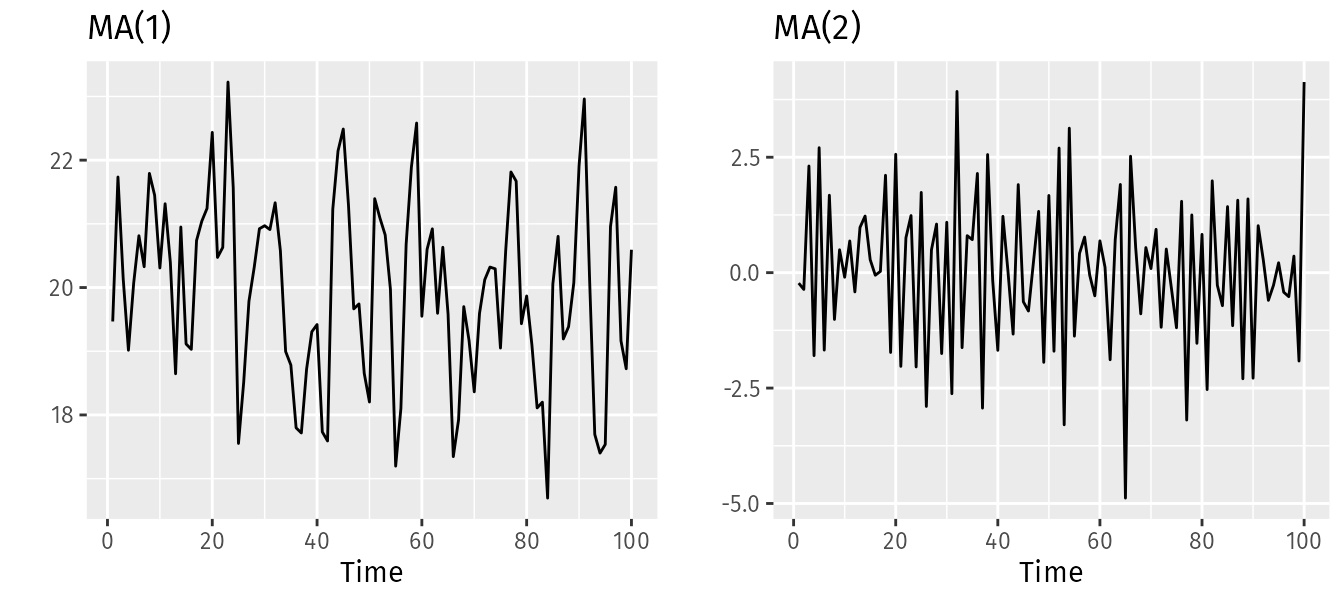
\includegraphics[width=\textwidth]{img/maq-1-example.png}        
        \end{minipage}
    
        \begin{minipage}[t]{0.9\textwidth}
            Fuente: Forecasting: Principles and Practice (Hyndman y Athanasopoulos, 2023). Recuperado de \url{https://otexts.com/fpp2/time-plots.html}
        \end{minipage}
    \end{figure}

    El modelo MA(1) tiene como fórmula: $y_t=20+\varepsilon_t+0.8\varepsilon_t-1$ y el modelo MA(2) tiene como fórmula: $y_t=\varepsilon_t - \varepsilon_t-1 + 0.8\varepsilon_t-2$, en ambos casos $\varepsilon_t$ (ruido blanco) tiene una distribución normal, con promedio igual a 0 y varianza igual a 1 \cite{forecast-time-series-arima}.

    Un modelo AR($p$) estacionario es capaz de ser escrito como un modelo MA($\infty$), esto se puede demostrar para un modelo AR(1)luego de realizar repetidas sustituciones:
    \begin{equation*}
    \begin{split}
    y_t &=\phi_1y_t-1+\varepsilon_t\\  &=\phi_1(\phi_1y_t-2+\varepsilon_t-1)+\varepsilon_t\\ &=\phi^2_1y_t-2+\phi_1\varepsilon_t-1+\varepsilon_t\\ &=\phi^3_1y_t-3+\phi^2_1\varepsilon_t-2+\phi_1\varepsilon_t-1+\varepsilon_t
    \end{split}
    \end{equation*}

    Teniendo $-1>\phi_1<1$, el valor de $\phi^k_1$ irá disminuyendo a medida que $k$ siga creciendo, obteniendo un proceso MA($\infty$) \cite{forecast-time-series-arima}, este tipo de modelo se escribe de la siguiente manera:
    \begin{equation*}
        y_t=\varepsilon_t+\phi_1\varepsilon_t-1+\phi^2_1\varepsilon_t-2+\phi^3_1\varepsilon_t-3+...
    \end{equation*}

    También se puede realizar el proceso inverso, para obtener un modelo AR($\infty$) desde un modelo MA, si es que se definen ciertos limites. Este tipo de modelos que se pueden transcribir de MA a AR($\infty$) y AR a MA($\infty$), son llamados modelos \textbf{invertibles} \cite{forecast-time-series-arima}.
\end{itemize}

Combinando los modelos de diferenciación, autorregresivo y de media móvil obtenemos el modelo \textbf{ARIMA} \cite{forecast-time-series-arima}, este queda modelado de la siguiente manera:
\begin{equation*}
    y'_t=c+\phi_1y'_t-1+...+\phi_py'_t-p+\theta_1\varepsilon_t-1+...+\theta_q\varepsilon_t-q+\varepsilon_t
\end{equation*}

Teniendo en cuenta que $y'_t$ corresponde a la serie diferenciada, a la derecha de la igualdad se encuentran las variables que permiten realizar las predicciones, entre estas se encuentran valores desfasados de $y_t$ y errores desfasados.
El modelo \textbf{ARIMA($p,d,q$)} tiene 3 variables, donde cada una de estas variables esta relacionada a \cite{forecast-time-series-arima}:
\begin{itemize}
    \item $p$ = orden de la parte autorregresiva del modelo.
    \item $d$ = grado de la primera diferenciación.
    \item $q$ = orden de la parte de media móvil.
\end{itemize}

De la misma manera que la estacionariedad e invertibilidad se aplican a los modelos de autorregresión y de media móvil, también se aplican para los modelos ARIMA. Este modelo presenta casos especiales, los cuales representan modelos anteriormente mencionados, los cuales son:
\begin{itemize}
    \item White noise: ARIMA(0,0,0)
    \item Random walk: ARIMA(0,1,0) sin constante
    \item Random walk con desfase: ARIMA(0,1,0) con constante
    \item Autorregresión: ARIMA($p$,0,0)
    \item Media móvil: ARIMA(0,0,$q$)
\end{itemize}
